% !TEX program = xelatex
% !BIB program = bibtex

\documentclass[UTF8]{article}

% layout
\usepackage[left=3cm,right=3cm]{geometry}
\linespread{1.25}
% \makeatletter
% \def\@seccntformat#1{%
%   \expandafter\ifx\csname c@#1\endcsname\c@section
%   Section \thesection:
%   \else
%   \csname the#1\endcsname\quad
%   \fi}
% \makeatother
 
% page headings
\usepackage{fancyhdr}
\setlength{\headheight}{15.2pt}
\pagestyle{fancy}
\lhead{\leftmark}
\rhead{M201873026 Yilong Liu}
\cfoot{\thepage}
% \makeatletter
% \let\headauthor\@author
% \makeatother

% url/ref
\usepackage{hyperref}
\hypersetup{
  colorlinks,
  citecolor=black,
  filecolor=black,
  linkcolor=black,
  urlcolor=black,
  pdfauthor={Yilong Liu},
  pdftitle={Dataflow architecture: state-of-the-art and research challenges}
}

% vertical centering title page
\usepackage{titling}
\renewcommand\maketitlehooka{\null\mbox{}\vfill}
\renewcommand\maketitlehookd{\vfill\null}

% table of contents
\usepackage{tocloft}
\renewcommand\cftsecfont{\normalfont}
\renewcommand\cftsecpagefont{\normalfont}
\renewcommand{\cftsecleader}{\cftdotfill{\cftsecdotsep}}
\renewcommand\cftsecdotsep{\cftdot}
\renewcommand\cftsubsecdotsep{\cftdot}
\renewcommand{\contentsname}{\hfill\bfseries\Large Contents\hfill}   
\setlength{\cftbeforesecskip}{10pt}

% figures
\usepackage{graphicx}
\graphicspath{figures/}
% \newcommand\figureht{\dimexpr
%   \textheight-3\baselineskip-\parskip-.2em-
%   \abovecaptionskip-\belowcaptionskip\relax}

% tables
\usepackage{caption} 
\captionsetup[table]{skip=10pt}

% math, algorithms, code
\usepackage{amsmath,amssymb,url}
\usepackage{algorithm,algorithmicx,algpseudocode}
\usepackage{listings}

\lstset{
   extendedchars=true,
   basicstyle=\footnotesize\ttfamily,
   showstringspaces=false,
   showspaces=false,
   numbers=left,
   numberstyle=\footnotesize,
   numbersep=9pt,
   tabsize=2,
   breaklines=true,
   showtabs=false,
   captionpos=b
}

% bibliography
\usepackage[super,square,comma,sort]{natbib} % for \citet and \citep
\renewcommand{\refname}{References}
% \begin{filecontents}{report.bib}
% \end{filecontents} 

% appendix
\usepackage{appendix}

\title{Survey \\ \bigskip \textbf{Dataflow architecture: state-of-the-art and research challenges}}
\author{School of computer science and technology\\ M1801\\ M201873026\\ Yilong Liu}
\date{\today}

\begin{document}

\pagenumbering{gobble} % no page number
\maketitle
\newpage
% \null\thispagestyle{empty}
% \newpage

% \pagenumbering{roman}
% \section*{Abstract}\sectionmark{Abstract}
% \addcontentsline{toc}{section}{Abstract}
% \addcontentsline{toc}{section}{\protect\numberline{}Abstract}
% \newpage
% \pagenumbering{gobble} % no page number

\tableofcontents
\newpage
% \null\thispagestyle{empty}
% \newpage

\pagenumbering{arabic}

\section{Introduction}
Dataflow architecture is a computer architecture that
directly contrasts the traditional von Neumann architecture
or control flow architecture.
Dataflow architectures do not have a program counter,
or (at least conceptually) the executability
and execution of instructions is solely determined
based on the availability of input arguments to the instructions,
so that the order of instruction execution is unpredictable.

\section{Dataflow Architecture}
Survey of basic dataflow architecture.

Dennis~\cite{DBLP:conf/isca/DennisM74} proposed ``The Elementary Processor'',
as figure~\ref{fig:elementory_processor}.
When a Cell contains an instruction and the necessary operands,
it is enabled and signals the Arbitration Network
that it is ready to transmit its contents as an operationace
to an Operation Unit which can perform the desired function.
The result of an operation leaves an Operation Unit
as one or more data packet,
consisting of the computed value and the address of a register
in the Memory to which the value is to be delivered.
The Dist£ibution Network accepts data packets
from the Operation Units and utilizes the address of each
to direct the data item through the network to the correct register in the Memory.
The Instruction Cell containing that register may then be enabled
if an instruction and all operands are present in the Cell.

\begin{figure}[htb]
  \begin{small}
    \begin{center}
      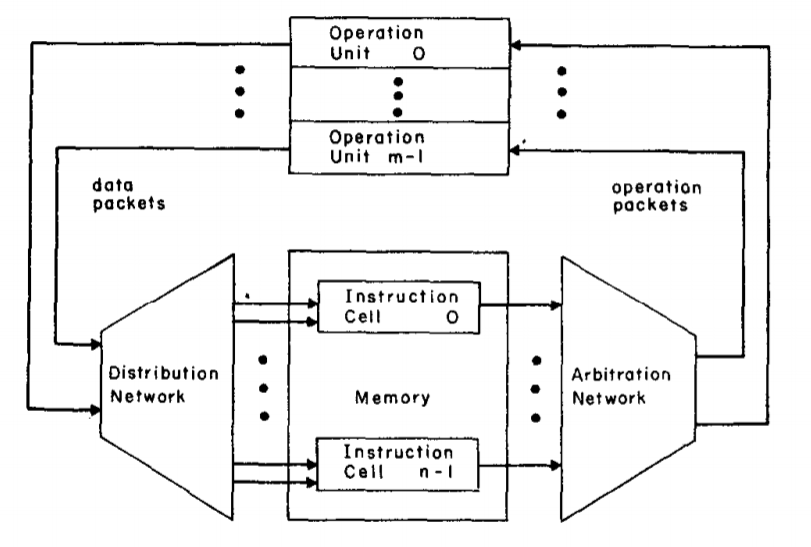
\includegraphics[width=\textwidth,height=8cm]{figures/isca94_elementory_processor.png}
    \end{center}
    \caption{ISCA94 - Elementary Processor.}
    \label{fig:elementory_processor}
  \end{small}
\end{figure}

Treleaven had a survey of dataflow architecture~\cite{DBLP:journals/csur/TreleavenBH82}.

\clearpage

% \begin{table}
%   \begin{small}    
%     \caption{This is for long caption.}
%     \label{tab:table}
%     \begin{center}
%       \begin{tabular}[c]{l|l}
%         \hline
%         \multicolumn{1}{c|}{\textbf{xx}} & 
%         \multicolumn{1}{c}{\textbf{xx}} \\
%         \hline
% 	      a & b \\
% 	      c & d \\
% 	      e & f \\
%         \hline
%       \end{tabular}
%     \end{center}
%   \end{small}
% \end{table}

% \begin{algorithm}
%   \floatname{algorithm}{算法}
% 	\algrenewcommand\algorithmicrequire{\textbf{输入:}}
% 	\algrenewcommand\algorithmicensure{\textbf{输出:}}
% 	\caption{xxxxxxxxxx}
% 	\label{alg:main}
%   \begin{algorithmic}[1]
%     \State \textbf{return} $state$
% 	\end{algorithmic}  
% \end{algorithm}

% \begin{equation}
%   \text{UCT} = \frac{w_i}{s_i} + c\sqrt{\frac{\ln{s_p}}{s_i}}
%   \label{eq:uct}
% \end{equation}

\bibliographystyle{unsrt}
\bibliography{bibs/dataflow}
\addcontentsline{toc}{section}{References}
\newpage

\end{document}
